\ProvidesFile{rutitlepage.dtx}[2022/02/21 v3.0 Radboud University Titlepage]
\documentclass{ltxdoc}
\newcommand{\messagespace}{\text{$\mathcal{M}$}}
\newcommand{\messageinstance}{\text{$m$}}
\newcommand{\ciphertextspace}{\text{$\mathcal{C}$}}
\newcommand{\ciphertextinstance}{\text{$c$}}
\newcommand{\associateddataspace}{\text{$\mathcal{A}$}}
\newcommand{\associateddatainstance}{\text{$a$}}
\newcommand{\tagspace}{\text{$\mathcal{T}$}}
\newcommand{\taginstance}{\text{$t$}}
\newcommand{\keyspace}{\text{$\mathcal{K}$}}
\newcommand{\keyinstance}{\text{$k$}}
\newcommand{\noncespace}{\text{$\mathcal{N}$}}
\newcommand{\nonceinstance}{\text{$n$}}
\newcommand{\lockspace}{\text{$\mathcal{L}$}}
\newcommand{\lockinstance}{\text{$l$}}
\newcommand{\users}{\text{$N$}}
\newcommand{\user}{\text{$j$}}
\newcommand{\adversary}{\text{$A$}}
\newcommand{\sample}{\text{$\leftarrow$}}
\newcommand{\result}{\text{$\leftarrow$}}
\newcommand{\concatinate}{\text{$\|$}}

\newcommand{\advantage}[2]{\textbf{Adv}$_{\text{#1}}^{\text{#2}}$ }
\newcommand{\probabilityblock}[4]{\text{$|\text{Pr}[\text{#1}_{\text{#2}}^{\text{#3}}] - \text{Pr}[\text{#1}_{\text{#2}}^{\text{#4}}]|$}}

\newcommand{\pkc}{\text{Hybrid Encryption in a Multi-user Setting, revised}}
\newcommand{\gcrec}{\text{Generic Composition Reconsidered}}

\newcommand{\x}{\text{x}}
\usepackage{a4wide}
\usepackage{float}
\usepackage{graphicx}
\usepackage{array}
\usepackage[utf8]{inputenc}
\usepackage{rutitlepage}
\usepackage{fancyhdr}
\usepackage[style=ieee]{biblatex}
\usepackage{cryptocode}
\usepackage{amssymb}
\addbibresource{cryptobib/crypto.bib}
\GetFileInfo{rutitlepage.dtx}

\pagestyle{fancy}
\fancyhf{}
\lhead{Bacholer Thesis}
\rhead{Page \thepage}

\title{research proposal}
\author{stijnvandenput }
\date{20 May 2022}

\begin{document}
\maketitleru[
    layout=traditional,
    authors={Stijn Vandenput},
    authorstext={Author:},
    nextpagenr={-1},
    date={20/05/2022},
    institution={Radboud Honours Academy},
    others={Supervisor:}{Martijn Stam\\Bart Mennink},
    course={Bachelor Thesis},
    title={TBD}]

\section*{Abstract}

\pagenumbering{roman}
\newpage
\tableofcontents

\newpage
\pagenumbering{arabic}

\section{Introduction}
should consist of:
\begin{itemize}
	\item explaining the challenge
	\item my contribution
\end{itemize}
Within the field of cryptography there are a two different fields, symmetric and asymmetric crypto. The former is about situations where the users have a shared secret already, the latter is about situations where this is not the case. Sometimes work in asymmetric crypto uses constructions that are more common in symmetric crypto, and in this fashion, \pkc{} uses a construction that is very similar to Authenticated Encryption following the generic encrypt-then-MAC construction. This construction has since been revised in \gcrec{} to be better applicable to common use cases. The aim of this thesis is to apply the knowledge of \gcrec{} to the setting of \pkc{} and in doing so, create a better primitive for authenticated encryption in a asymmetric crypto setting.

\section{Preliminaries}
should consist of:
\begin{itemize}
    \item general notation
    \item generic AE construction
	\item generic PKE schemes
	\item nonces vs locks
\end{itemize}

\subsection{notation table}
\begin{tabular}{|c | c | c | c | m{5cm}|}
    \hline
    Name   &   pkc   &   GCrec   &   my notation & rough meaning \\[0.5 ex]
    \hline
    \hline
    message space   &   $\mathcal{M}$   &   $\mathcal{M}$   &   \messagespace & set of all possible message options \\
    \hline
    message   &   $m$   &   $M$   &   \messageinstance &  message the user sends \\
    \hline
    ciphertext space   &   $\mathcal{C}$   &   -   &   \ciphertextspace & set of all possible ciphertext options \\
    \hline
    ciphertext   &   $c$   &   $C$   &   \ciphertextinstance & encrypted message \\
    \hline
    associated data space   &   -   &   $\mathcal{A}$   &   \associateddataspace & set of all possible associated data options \\
    \hline
    associated data   &   -   &   $A$   &   \associateddatainstance & data you want to authenticate but not encrypt \\
    \hline
    tag space   &   $\mathcal{C}$   &   $\mathcal{T}$   &   \tagspace & set off all possible tag options \\
    \hline
    tag   &   $c$   &   $T$   &   \taginstance & output of mac function \\
    \hline
    key space   &   $\mathcal{K}$   &   $\mathcal{K}$   &   \keyspace & set of all possible key options \\
    \hline
    key   &   $k$   &   $K$   &   \keyinstance   & user key \\
    \hline
    nonce space   &   -   &   $\mathcal{N}$   &   \noncespace & set of all nonce options \\
    \hline
    nonce   &   -   &   $n$   &   \nonceinstance & number only used once \\
    \hline
    lock space   &   $\mathcal{T}$   &   -   &   \lockspace & set of all possible lock options \\
    \hline
    lock   &   $t$   &   -   &   \lockinstance & nonce that is bound to the user \\
    \hline
    users   &   $N$   &   -   &   \users & number of users \\
    \hline
    adversary   &   A   &   $\mathcal{A}$   &   \adversary & the bad guy \\
    \hline
    Random sampling   &   $\leftarrow^{\$}$    &   $\twoheadleftarrow$   &   \sample & get a random ellermetn form the set \\
    \hline
    result of function   &   $\leftarrow^{\$}$   &   $\leftarrow$   &   \result & get the result of a function with given inputs \\
    \hline
    concatination   &   a$\|$b   &   a$\|$b   &   a\concatinate{}b & concatanation of two strings \\
    %Name   &   pkc   &   GCrec   &   my notation & rough meaning \\
    %\hline
    \hline
\end{tabular}

\section{Existing AE/DEM notations in more detail}
should consist of:
\begin{itemize}
	\item the definition of the two paper, if possible already brought more toward one notation standard
	\item explain how both relate to the preliminaries and overall story
\end{itemize}

\subsection{Existing notation from \pkc}
\subsubsection{notation}
\messagespace{} is a message space, \keyspace{} is a finite key space, \lockspace{} is a lock space and \ciphertextspace{} is a ciphertext space. \users{} is the number of users.
\subsubsection{used primitives}
\begin{itemize}
    \item ADEM: the ADEM exists of tuple (A.enc,A.dec), A.enc take a key \keyinstance{} in \keyspace{}, a lock \lockinstance{} in \lockspace{} and a message \messageinstance{} in \messagespace{} and outputs a ciphertext \ciphertextinstance{} in \ciphertextspace{}. A.dec takes a \keyinstance{} in \keyspace{}, a lock \lockinstance{} in \lockspace{} and a ciphertext \ciphertextinstance{} in \ciphertextspace{} and outputs a message \messageinstance{} in \messagespace{} or $\bot$ to indicate rejection. The correctness requirement is that for every combination of \keyinstance{}, \lockinstance{} and \messageinstance{} we have A.dec(\keyinstance,\lockinstance,A.enc(\keyinstance,\lockinstance,\messageinstance)) = \messageinstance. The security of the ADEM is defined with \advantage{ADEM,\adversary,\users}{n-moit-ind} = \probabilityblock{N-MIOT-IND}{\adversary,\users}{0}{1}, defined by the following game:
    \begin{figure}[H]
        \centering
        \begin{pchstack}[boxed,center,space=0.5cm]
            \pseudocode[lnstart=-1,linenumbering,head={\textbf{Game} N-MOIT-IND$^{b}_{\adversary,\users}$ }]{
            L = \emptyset\\
            \pcfor \user \in [1..N]:\\
            \t \keyinstance_\user \sample \keyspace\\
            \t C_\user = \emptyset\\
            b' \result \adversary\\
            \pcreturn b'
            }
            \pseudocode[lnstart=5,linenumbering,head={\textbf{Oracle} Oenc(\user,\lockinstance,\messageinstance$_0$,\messageinstance$_1$)}]{
                \pcif C_\user \neq \emptyset: \pcreturn \bot\\
                \pcif \lockinstance \in L: \pcreturn \bot\\
                L = L \cup \{\lockinstance\}\\
                \lockinstance_\user = \lockinstance\\
                \ciphertextinstance \result \text{A.enc}(\keyinstance_\user,\lockinstance_\user,\messageinstance_b)\\
                C_\user = \ciphertextinstance\\
                \pcreturn \ciphertextinstance
            }
            \pseudocode[lnstart=12,linenumbering,head={\textbf{Oracle} Odec(\user,\ciphertextinstance)}]{
                \pcif C_\user \neq \emptyset: \pcreturn \bot\\
                \pcif \ciphertextinstance \in C_\user: \pcreturn \bot\\
                \messageinstance \result \text{A.dec}(\keyinstance_\user,\lockinstance_\user,\ciphertextinstance)\\
                \pcreturn \messageinstance
            }
        \end{pchstack}
        \caption{N-MIOT-IND game, \adversary{} has access to oracles Oenc and Odec and the tags in line 10 and 15 are the same.}
    \end{figure}
    
    \item AMAC: the AMAC exists of tuple (M.mac,M.vrf). M.mac takes a key \keyinstance{} in \keyspace{}, a lock \lockinstance{} in \lockspace{}, and a message \messageinstance{} in \messagespace{} and outputs a ciphertext \ciphertextinstance{} in \ciphertextspace{}. M.vrf takes a key \keyinstance{} in \keyspace{}, a lock \lockinstance{} in \lockspace{}, a message \messageinstance{} in \messagespace{} and a ciphertext \ciphertextinstance{} in \ciphertextspace{} and returns either $true$ of $false$. The correctness requirement is that for every combination of \keyinstance{}, \lockinstance{} and \messageinstance{}, all corresponding \ciphertextinstance{} \result M.mac(\keyinstance,\lockinstance,\messageinstance) gives M.vrf(\keyinstance,\lockinstance,\messageinstance,\ciphertextinstance)=$true$. The security of the AMAC is defined with \advantage{AMAC,\adversary,\users}{N-MIOT-UF} = \probabilityblock{N-MIOT-UF}{\adversary,\users}{0}{1}, defined by the following game:
    \begin{figure}[H]
        \centering
        \begin{pchstack}[boxed,center,space=0.5cm]
            \pseudocode[lnstart=-1,linenumbering,head={\textbf{Game} N-MIOT-UF$^{b}_{\adversary,\users}$ }]{
            L = \emptyset\\
            \pcfor \user \in [1..N]:\\
            \t \keyinstance_\user \sample \keyspace\\
            \t T_\user = \emptyset\\
            b' \result \adversary\\
            \pcreturn b'
            }
            \pseudocode[lnstart=5,linenumbering,head={\textbf{Oracle} Omac(\user,\lockinstance,\messageinstance$_0$,\messageinstance$_1$)}]{
                \pcif T_\user \neq \emptyset: \pcreturn \bot\\
                \pcif \lockinstance \in L: \pcreturn \bot\\
                L = L \cup \{\lockinstance\}\\
                \lockinstance_\user = \lockinstance\\
                \taginstance \result \text{M.mac}(\keyinstance_\user,\lockinstance_\user,\messageinstance_b)\\
                T_\user = (\messageinstance,\taginstance)\\
                \pcreturn \taginstance
            }
            \pseudocode[lnstart=12,linenumbering,head={\textbf{Oracle} Ovrf(\user,\messageinstance,\taginstance)}]{
                \pcif T_\user \neq \emptyset: \pcreturn \bot\\
                \pcif (\messageinstance,\taginstance) \in T_\user: \pcreturn \bot\\
                \pcif \text{M.vrf}(\keyinstance_\user,\lockinstance_\user,\messageinstance,\taginstance): \\
                \t \pcreturn true\\
                \pcelse : \pcreturn false
            }
        \end{pchstack}
        \caption{N-MIOT-UF game, \adversary{} has access to oracles Omac and Ovrf and the tags in line 10 and 15 are the same.}
    \end{figure}
\end{itemize}

\subsubsection{goal}
The goal is to make a scheme ADEM' from the ADEM and AMAC which has the same security of the ADEM, but is also secure against active attacks.

\subsubsection{Security model}
The security is defined by creating new A.enc' and A.dec' calls which are build using the calls the primitives provide us, and placing those in the ADEM game defined earlier:
\begin{figure}[H]
    \centering
    \begin{pchstack}[boxed,center,space=0.5cm]
        \pseudocode[lnstart=-1,linenumbering,head={\textbf{Proc} A.enc'(\keyinstance,\lockinstance,\messageinstance)}]{
        (\keyinstance_{dem},\keyinstance_{mac}) \result \keyinstance\\
        \ciphertextinstance' \result \text{A.enc}(\keyinstance_{dem},\lockinstance,\messageinstance)\\
        \taginstance \result \text{M.mac}(\keyinstance_{mac},\lockinstance,\ciphertextinstance')\\
        \ciphertextinstance \result (\ciphertextinstance',\taginstance)\\
        \pcreturn \ciphertextinstance
        }
        \pseudocode[lnstart=5,linenumbering,head={\textbf{Proc} A.dec'(\keyinstance,\lockinstance,\ciphertextinstance)}]{
            (\keyinstance_{dem},\keyinstance_{mac}) \result \keyinstance\\
            (\ciphertextinstance',\taginstance) \result \ciphertextinstance\\
            \pcif \text{M.mac}(\keyinstance_{mac},\lockinstance,\ciphertextinstance',\taginstance):\\
            \t \messageinstance \result \text{A.dec}(\keyinstance_{dem},\lockinstance,\ciphertextinstance')\\
            \t \pcreturn \messageinstance\\
            \pcelse : \pcreturn \bot
        }
    \end{pchstack}
    \caption{A.enc' and A.dec' calls}
\end{figure}
\noindent The new advantage is \advantage{ADEM',$A$,\users}{n-miot} $\leq$ 2\advantage{AMAC,$B$,\users}{n-miot-uf} + \advantage{ADAM,$C$,\users}{n-moit-ind}. Where the running time of $B$ is at most that of $A$ plus the time required to run \users-many ADEM encapsulations and Qd-many ADEM decapsulations and the running time of $C$ is the same as the running time of $A$. Additionally, $B$ poses at most Qd-many Ovrf queries, and $C$ poses no Odec query.

\subsection{Existing notation from \gcrec}
\subsubsection{notation}
\keyspace{} is a nonempty key space, \noncespace{} is a non-empty nonce space, \messagespace{} is a message space and \associateddataspace{} is the associated-data space. \messagespace{} contain at least two strings, and if \messagespace{} and \associateddataspace{} contain a string of length x, they must contain all strings of length x.

\subsubsection{used primitives}
\begin{itemize}
    \item nE: A nonce-based E scheme is defined by triple (\keyspace{},E,D). E is a deterministic encryption algorithm that takes three inputs (K,N,M) to a value C, the length of C only depends the length of K, N and M. When (K,N,M) is not in $\keyspace \times \noncespace \times \messagespace$, C will be $\bot$. D is the decryption algorithm that takes three inputs (K,N,C) to a value M. E and D are inverse of each other implying correctness (if E(K,N,M) $= C \neq \bot$, then D(K,N,C) = M) and tidiness (if D(K,N,C) $= M \neq \bot$, then E(K,N,M) = C). The security is defined as follows:\\ \fbox{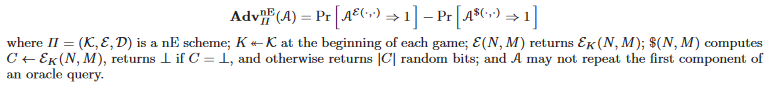
\includegraphics[scale = 0.8]{images/sec nE.png}}
    \item MAC: The MAC is a deterministic algorithm F that takes in a K in \keyspace{} and a string x and outputs either a n-bit length T or $\bot$. The domain of F is the set X such that F(K,x) $\neq \bot$. The security of F is defined by \advantage{F}{pfr} =\probabilityblock{A}{}{F}{p}. the game on the left selects a random K from \keyspace{} and provides oracle access to F(K,.) the game on the right selects a uniformly random function p from X to \{1,0\}$^n$ and provide oracle access to it. With each oracle, queries outside X return $\bot$
\end{itemize}

\subsubsection{goal}
The end goal is a nonce-based authenticated encryption scheme (\keyspace{},E,D). E is a deterministic encryption algorithm that takes four inputs (K,N,A,M) to a value C, the length of C value only depends the length of K, N, A and M. When (K,N,A,M) is not in $\keyspace \times \noncespace \times \associateddataspace \times \messagespace$, C will be $\bot$. D is the decryption algorithm that takes four inputs (K,N,A,C) to a value M. E and D are inverse of each other implying correctness (if E(K,N,A,M) $= C \neq \bot$, then D(K,N,A,C) = M) and tidiness (if D(K,N,A,C) $= M \neq \bot$, then E(K,N,A,M) = C)
\subsubsection{Security model}
Security is defined as follows: \\ \fbox{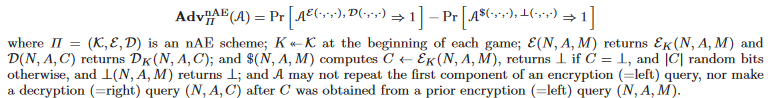
\includegraphics[scale = 0.88]{images/sec nAE.png}}\\
We define the scheme secure if there is a tight reduction from breaking the nAE-security of the scheme to breaking the nE-security and the PRF security of the underlying primitives.

\section{New Definition}
should consist of:
\begin{itemize}
	\item syntax of the primitive (input,output,correctness,tidiness, expected bounds)
	\item game based code
	\item explanation of the choices made
	\item formal comparison with other choices
\end{itemize}

\subsection{notation}
\keyspace{} is a nonempty key space, \lockspace{} is a non-empty lock space and \messagespace{} is a message space. \messagespace{} contain at least two strings, and if it contain a string of length x, it must contain all strings of length x. \users is the number of users.

\subsection{goal}
The end goal is to build a Authenticated Encryption scheme (EA). The AE scheme is defined by tuple (AE.enc,AE.dec). AE.enc is a deterministic encryption algorithm that takes three inputs (\keyinstance,\lockinstance,\messageinstance) to a value \ciphertextinstance, the length of \ciphertextinstance{} only depends on the length of \keyinstance, \lockinstance{} and \messageinstance. When (\keyinstance,\lockinstance,\messageinstance) is not in $\keyspace \times \lockspace \times \messagespace$, \ciphertextinstance{} will be $\bot$. AE.dec is the decryption algorithm that takes three inputs (\keyinstance,n,\ciphertextinstance) to a value \messageinstance. AE.enc and E.dec are inverse of each other implying correctness (if AE.enc(\keyinstance,\lockinstance,\messageinstance) $= \ciphertextinstance \neq \bot$, then AE.dec(\keyinstance,\lockinstance,\ciphertextinstance) = \messageinstance) and tidiness (if AE.dec(\keyinstance,\lockinstance,\ciphertextinstance) $= \messageinstance \neq \bot$, then AE.enc(\keyinstance,\lockinstance,\messageinstance) = \ciphertextinstance).

\subsection{Security model}
The advantage is calculated with \advantage{\adversary,\users}{AE} = \probabilityblock{AE}{\adversary,\users}{AE}{\$}. AE$^{\text{AE}}_{\adversary,\users}$ is defined below, AE$^{\$}_{\adversary,\users}$is the game AE$^{\text{AE}}_{\adversary,\users}$, where AE.enc in line 10 is replaced with \$.enc. \$.enc(\keyinstance,\lockinstance,\messageinstance) calls \ciphertextinstance{} = AE.enc(\keyinstance,\lockinstance,\messageinstance) then outputs $\bot$ if \ciphertextinstance{} is $\bot$ or $\mid \ciphertextinstance \mid$ random bits otherwise. EA.dec in line 15 is replaced with \$.dec(\keyinstance,\lockinstance,\ciphertextinstance) that always returns $\bot$
\begin{figure}[H]
    \begin{pchstack}[boxed,center,space=0.5cm]
        \pseudocode[lnstart=-1,linenumbering,head={\textbf{Game} AE$^{AE}_{\adversary,\users}$ }]{
        L = \emptyset\\
        \pcfor \user \in [1..N]:\\
        \t \keyinstance_\user \sample \keyspace\\
        \t C_\user = \emptyset\\
        b' \result \adversary\\
        \pcreturn b'
        }
        \pseudocode[lnstart=5,linenumbering,head={\textbf{Oracle} Oenc(\user,\lockinstance,\messageinstance)}]{
            \pcif C_\user \neq \emptyset: \pcreturn \bot\\
            \pcif \lockinstance \in L: \pcreturn \bot\\
            L = L \cup \{\lockinstance\}\\
            \lockinstance_\user = \lockinstance\\
            \ciphertextinstance \result \text{AE.enc}(\keyinstance_\user,\lockinstance_\user,\messageinstance)\\
            C_\user = \ciphertextinstance\\
            \pcreturn \ciphertextinstance
        }
        \pseudocode[lnstart=12,linenumbering,head={\textbf{Oracle} Odec(\user,\ciphertextinstance)}]{
            \pcif C_\user \neq \emptyset: \pcreturn \bot\\
            \pcif \ciphertextinstance \in C_\user: \pcreturn \bot\\
            \messageinstance \result \text{AE.dec}(\keyinstance_\user,\lockinstance_\user,\ciphertextinstance)\\
            \pcreturn \messageinstance
        }
    \end{pchstack}
    \caption{AE game}
\end{figure}

\subsection{choices made}
In this security model, there are a lot of choices made, in this section I will elaborate on these. Firstly, the used MAC primitive is required to be indistinguishable from RO. This choice was made as it is required for AE constructions from \gcrec{}. I also choose to have "locks" instead of nonces. In this setting, this results in the adversary not being able to make decryption queries for any incorrect lock values. I choose this as a setting with locks will suffice the setting of hybrid encryption while probably being easier to prove. For this reason I also choose to not allow multiple encryption calls for one user, as well as not allowing decryption calls to a user which encryption call is not yet made. In my security game for the DEM, there is no decryption oracle considered. When distinguishing from a random function, this is equivalent to a situation in which a decryption oracle is considered (I am not 100\% sure about his part). Lastly, we choose to indistinguishably from a random function as a security model, instead of indistinguishably of two encrypted messages. This is a stronger security notion in the current setting as the length of the ciphertext only depends on the length of the inputs. Indistinguishably of two encrypted messages probably suffices in the current setting so I might still change to this if proving indistinguishably from a random function seems infeasible.

\section{Constructions}
should consist of:
\begin{itemize}
    \item the old primitives
	\item how to construct the new primitive from old primitives
	\item security bounds + proof
	\item comparison with existing alternatives
\end{itemize}

\subsection{used primitives}
\keyspace{} is a nonempty key space, \noncespace{} is a non-empty nonce space and \messagespace{} is a message space. \messagespace{} contain at least two strings, and if it contain a string of length x, it must contain all strings of length x. \users is the number of users.
\begin{itemize}
    \item DEM: a DEM scheme is defined by tuple (E.enc,E.dec). E.enc is a deterministic encryption algorithm that takes three inputs (\keyinstance,\lockinstance,\messageinstance) to a value \ciphertextinstance, the length of \ciphertextinstance{} only depends on the length of \keyinstance, \lockinstance{} and \messageinstance. When (\keyinstance,\lockinstance,\messageinstance) is not in $\keyspace \times \lockspace \times \messagespace$, \ciphertextinstance{} will be $\bot$. E.dec is the decryption algorithm that takes three inputs (\keyinstance,\lockinstance,\ciphertextinstance) to a value \messageinstance. E.enc and E.dec are inverse of each other implying correctness (if E.enc(\keyinstance,\lockinstance,\messageinstance) $= \ciphertextinstance \neq \bot$, then E.dec(\keyinstance,\lockinstance,\ciphertextinstance) = \messageinstance) and tidiness (if E.dec(\keyinstance,\lockinstance,\ciphertextinstance) $= \messageinstance \neq \bot$, then E.enc(\keyinstance,\lockinstance,\messageinstance) = \ciphertextinstance). The advantage is calculated with \advantage{\adversary,\users}{DEM} = \probabilityblock{DEM}{\adversary,\users}{DEM}{\$}. DEM$^{\text{DEM}}_{\adversary,\users}$ is defined below, DEM$^{\$}_{\adversary,\users}$is the game DEM$^{\text{DEM}}_{\adversary,\users}$, where E.enc in line 10 is replaced with \$.enc(\keyinstance,\lockinstance,\messageinstance). \$.enc calls \ciphertextinstance{} = E.enc(\keyinstance,\lockinstance,\messageinstance) then outputs $\bot$ if \ciphertextinstance{} is $\bot$ or $\mid \ciphertextinstance \mid$ random bits otherwise.
    \begin{figure}[H]
        \begin{pchstack}[boxed,center,space=0.5cm]
            \pseudocode[lnstart=-1,linenumbering,head={\textbf{Game} DEM$^{\text{DEM}}_{\adversary,\users}$ }]{
            L = \emptyset\\
            \pcfor \user \in [1..\users]:\\
            \t \keyinstance{}_\user \sample \keyspace\\
            \t C_\user = \emptyset\\
            b' \result \adversary\\
            \pcreturn b'
            }
            \pseudocode[lnstart=5,linenumbering,head={\textbf{Oracle} Oenc(\user,\lockinstance,\messageinstance)}]{
                \pcif C_\user \neq \emptyset: \pcreturn \bot\\
                \pcif \lockinstance \in L: \pcreturn \bot\\
                L = L \cup \{\lockinstance\}\\
                \lockinstance{}_\user = \lockinstance\\
                \ciphertextinstance \result \text{E.enc}(\keyinstance{}_\user,\lockinstance{}_\user,\messageinstance)\\
                C_\user = \ciphertextinstance\\
                \pcreturn \ciphertextinstance
            }
        \end{pchstack}
    \caption{DEM game}
    \end{figure} 
    
    \item MAC: The MAC is a deterministic algorithm M.mac that takes in a fixed length \keyinstance in \keyspace{}, a fixed length \lockinstance{} in \lockspace{} and a variable length message \messageinstance{} in \messagespace{} and outputs either a n-bit length tag or $\bot$. The domain of M.mac is the set X such that M.mac(\keyinstance,\lockinstance,\messageinstance) $\neq \bot$. The advantage is calculated with \advantage{\adversary,\users}{MAC} = \probabilityblock{MAC}{\adversary,\users}{MAC}{\$}. MAC$^{\text{MAC}}_{\adversary,\users}$ is defined below, MAC$^{\$}_{\adversary,\users}$is the game MAC$^{\text{MAC}}_{\adversary,\users}$, where M.mac in line 10 is replaced with \$.mac. \$.mac(\keyinstance,\lockinstance,\messageinstance) computes \taginstance{} = M.mac(\keyinstance,\lockinstance,\messageinstance) then outputs $\bot$ if \taginstance{} is $\bot$ or $\mid \taginstance \mid$ random bits otherwise.
    \begin{figure}[H]
        \begin{pchstack}[boxed,center,space=0.5cm]
            \pseudocode[lnstart=-1,linenumbering,head={\textbf{Game} MAC$^{\text{MAC}}_{\adversary,\users}$ }]{
            L = \emptyset\\
            \pcfor \user \in [1..N]:\\
            \t \keyinstance_\user \sample \keyspace\\
            \t T_\user = \emptyset\\
            b' \result A\\
            \pcreturn b'
            }
            \pseudocode[lnstart=5,linenumbering,head={\textbf{Oracle} Omac(\user,\lockinstance,\messageinstance)}]{
                \pcif T_\user \neq \emptyset: \pcreturn \bot\\
                \pcif \lockinstance \in L: \pcreturn \bot\\
                L = L \cup \{\lockinstance\}\\
                \lockinstance_\user = \lockinstance\\
                \taginstance \leftarrow \text{M.mac}(\keyinstance_\user,\lockinstance_\user,\messageinstance)\\
                T_\user = \taginstance\\
                \pcreturn \taginstance
            }
        \end{pchstack}
    \caption{MAC game}
    \end{figure}
\end{itemize}

\subsection{construction}
The AE schemes we will look at are constructed from the DEM and the MAC. Following \gcrec{}, three ways to construct this AE are of interest, namely the ones following from the N1, N2 and N3 scheme. One thing to keep in mind with this that these schemes would originally use associated data. For now we can discard this but it is not proven that the same security results would also follow from this case without associated data. Down here the schemes, adjusted to our setting, can be found, followed by the AE.enc and AE.dec calls that can we construct following these schemes. These calls can be plugged into AE$^{\text{AE}}_{\adversary,\users}$ to find their respective security games.
\begin{figure}[H]
    \centering
    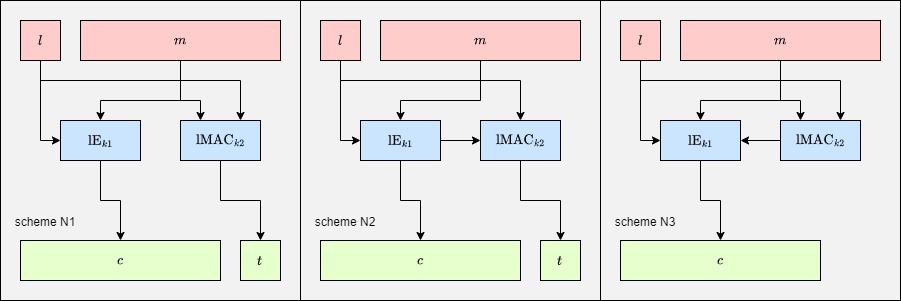
\includegraphics[scale = 0.4]{images/N-schemes.png}
\caption{Adjusted N schemes from \gcrec}
\end{figure}

\begin{figure}[H]
    \begin{pchstack}[boxed,center,space=0.5cm]
        \pseudocode[lnstart=-1,linenumbering,head={AE.enc(\keyinstance,\lockinstance,\messageinstance)}]{
            (\keyinstance{}1,\keyinstance{}2) \result \keyinstance \\
            \ciphertextinstance' \result \text{E.enc}(\keyinstance{}1,\lockinstance,\messageinstance) \\
            \taginstance \result \text{M.mac}(\keyinstance{}2,\lockinstance,\messageinstance) \\
            \ciphertextinstance \result (\ciphertextinstance',\taginstance)\\
            \pcreturn \ciphertextinstance
        }
        \pseudocode[lnstart=4,linenumbering,head={AE.dec(\keyinstance,\lockinstance,\ciphertextinstance)}]{
            (\keyinstance{}1,\keyinstance{}2) \result \keyinstance \\
            (\ciphertextinstance',\taginstance) \result \ciphertextinstance \\
            \messageinstance \result \text{E.dec}(\keyinstance{}1,\lockinstance,\ciphertextinstance') \\
            \taginstance' \result \text{M.mac}(\keyinstance{}2,\lockinstance,\messageinstance) \\
            \pcif \taginstance = \taginstance' : \pcreturn \messageinstance \\
            \pcelse : \pcreturn \bot
        }
    \end{pchstack}
\caption{Calls based on N1}
\end{figure}

\begin{figure}[H]
    \begin{pchstack}[boxed,center,space=0.5cm]
        \pseudocode[lnstart=-1,linenumbering,head={AE.enc(\keyinstance,\lockinstance,\messageinstance)}]{
            (\keyinstance{}1,\keyinstance{}2) \result \keyinstance\\
            \ciphertextinstance' \result \text{E.enc}(\keyinstance{}1,\lockinstance,\messageinstance)\\
            \taginstance \result \text{M.mac}(\keyinstance{}2,\lockinstance,\ciphertextinstance')\\
            \ciphertextinstance \result (\ciphertextinstance',\taginstance)\\
            \pcreturn \ciphertextinstance
        }
        \pseudocode[lnstart=4,linenumbering,head={AE.dec(\keyinstance,\lockinstance,\ciphertextinstance)}]{
            (\keyinstance{}1,\keyinstance{}2) \result \keyinstance\\
            (\ciphertextinstance',\taginstance) \result \ciphertextinstance\\
            \messageinstance \result \text{E.dec}(\keyinstance{}1,\lockinstance,\ciphertextinstance')\\
            \taginstance' \result \text{M.mac}(\keyinstance{}2,\lockinstance,\ciphertextinstance')\\
            \pcif \taginstance = \taginstance' : \pcreturn \messageinstance \\
            \pcelse : \pcreturn \bot
        }
    \end{pchstack}
\caption{Calls based on N2}
\end{figure}

\begin{figure}[H]
    \begin{pchstack}[boxed,center,space=0.5cm]
        \pseudocode[lnstart=-1,linenumbering,head={AE.enc(\keyinstance,\lockinstance,\messageinstance)}]{
            (\keyinstance{}1,\keyinstance{}2) \result \keyinstance\\
            \taginstance \result \text{M.mac}(\keyinstance{}2,\lockinstance,\messageinstance)\\
            \messageinstance' \result \messageinstance \concatinate \taginstance\\
            \ciphertextinstance \result E.enc(\keyinstance{}1,\lockinstance,\messageinstance')\\
            \pcreturn \ciphertextinstance
        }
        \pseudocode[lnstart=4,linenumbering,head={AE.dec(\keyinstance,\lockinstance,\ciphertextinstance)}]{
            (\keyinstance{}1,\keyinstance{}2) \result \keyinstance\\
            \messageinstance' \result \text{E.dec}(\keyinstance{}1,\lockinstance,\ciphertextinstance)\\
            (\messageinstance,\taginstance) \result \messageinstance'\\
            \taginstance' \result \text{M.mac}(\keyinstance{}2,\lockinstance,\messageinstance)\\
            \pcif \taginstance = \taginstance' : \pcreturn \messageinstance \\
            \pcelse : \pcreturn \bot
        }
    \end{pchstack}
\caption{Calls based on N3}
\end{figure}

The scheme is considered secure when there is a tight reduction from breaking the AE-security of the scheme to breaking the defined security of the underlying primitives.

\section{Use cases}
should consist of:
\begin{itemize}
	\item possible use cases
\end{itemize}

\section{Related Work}
\textbf{Location not final yet}

\section{Conclusion}

\newpage
\printbibliography[heading=bibintoc,title={References}]
\section{Appendix}

\end{document}

\NeedsTeXFormat{LaTeX2e}
\ProvidesPackage{rutitlepage}[2022/02/21 Mart Lubbers]
\RequirePackage{geometry,graphicx,ifpdf,keyval,iflang}
\def\@rutitleauthors{\@author}
\def\@rutitleauthorstext{Aut\IfLanguageName{dutch}{eu}{ho}r:}
\def\@rutitledate{\@date}
\def\@rutitleinst{Radboud Universit\IfLanguageName{dutch}{eit}{y} Nijmegen}
\def\@rutitletitle{\@title}
\def\@rutitlelayout{twentytwo}
\newif\if@rutitlecolour\@rutitlecolourfalse
\define@key{maketitleru}{authors}{\def\@rutitleauthors{#1}}
\define@key{maketitleru}{authorstext}{\def\@rutitleauthorstext{#1}}
\define@key{maketitleru}{colour}[true]{\@rutitlecolourtrue}
\define@key{maketitleru}{course}{\def\@rutitlecourse{#1}}
\define@key{maketitleru}{date}{\def\@rutitledate{#1}}
\define@key{maketitleru}{institution}{\def\@rutitleinst{#1}}
\define@key{maketitleru}{layout}{\def\@rutitlelayout{#1}}
\define@key{maketitleru}{nextpagenr}{\def\@rutitlenextpagenr{#1}}
\define@key{maketitleru}{others}{\def\@rutitleothers{#1}}
\define@key{maketitleru}{subtitle}{\def\@rutitlesubtitle{#1}}
\define@key{maketitleru}{title}{\def\@rutitletitle{#1}}
\newcommand*{\rutitlepage@printothers}[2]{\textit{#1}\\#2}
\newcommand*{\rutitlepage@sepothers}{\\[\baselineskip]}
\newcommand*{\rutitlepage@others}[2]{%
	\rutitlepage@printothers{#1}{#2}%
	\kernel@ifnextchar,{\rutitlepage@sepothers\rutitlepage@otherslist@}\relax}
\newcommand*{\rutitlepage@otherslist}[1]{%
	\expandafter\rutitlepage@others#1}
\def\rutitlepage@otherslist@,#1{\rutitlepage@otherslist{{#1}}}
\newcommand{\rutitle@layout@twentytwo}[0]{
	\newgeometry{left=25mm,top=25mm,right=15mm,bottom=10mm,hmarginratio=1:1}
	\begin{titlepage}%
		\null\vfill%
		\parindent0pt
		\ifdefined\@rutitlecourse\textsc{\LARGE\@rutitlecourse}\\[1.5cm]\fi
		{\Huge\bfseries\@rutitletitle}%
		\ifdefined\@rutitlesubtitle{\\[2\baselineskip]\large\itshape\@rutitlesubtitle\/}\fi\\[4\baselineskip]
		{\Large\scshape\@rutitleauthors}\\[\baselineskip]
		{\large\@rutitledate}
		\vfill

		\ifdefined\@rutitleothers\rutitlepage@otherslist\@rutitleothers\fi
		\vfill

		\hfill
		\ifpdf\includegraphics[width=80mm]{rutitlepage-logo-\IfLanguageName{dutch}{nl-}{}\if@rutitlecolour cmyk\else bw\fi.pdf}\\
		\else\includegraphics[width=80mm]{rutitlepage-logo-\IfLanguageName{dutch}{nl-}{}\if@rutitlecolour cmyk\else bw\fi.eps}\\
		\fi
	\end{titlepage}
	\restoregeometry%
}
\newcommand{\rutitle@layout@seventeen}[0]{
	\newgeometry{left=25mm,top=25mm,right=15mm,bottom=10mm,hmarginratio=1:1}
	\begin{titlepage}%
		\null\vfill%
		\parindent0pt
		{\Huge\bfseries\@rutitletitle}%
		\ifdefined\@rutitlesubtitle{\\[2\baselineskip]\large\itshape\@rutitlesubtitle\/}\fi\\[4\baselineskip]
		{\Large\scshape\@rutitleauthors}\\[\baselineskip]
		{\large\@rutitledate}
		\vfill

		\ifdefined\@rutitleothers\rutitlepage@otherslist\@rutitleothers\fi
		\vfill

		\hfill
		\ifpdf\includegraphics[width=80mm]{rutitlepage-logo-\IfLanguageName{dutch}{nl-}{}\if@rutitlecolour cmyk\else bw\fi.pdf}\\
		\else\includegraphics[width=80mm]{rutitlepage-logo-\IfLanguageName{dutch}{nl-}{}\if@rutitlecolour cmyk\else bw\fi.eps}\\
		\fi
	\end{titlepage}
	\restoregeometry%
}
\newcommand{\rutitle@layout@traditional}[0]{
	\newgeometry{hmarginratio=1:1}
	\begin{titlepage}
		\begin{center}
			\ifdefined\@rutitlecourse\textsc{\LARGE\@rutitlecourse}\\[1.5cm]\fi
			\ifpdf\includegraphics[height=150pt]{rutitlepage-logo.pdf}\\
			\else\includegraphics[height=150pt]{rutitlepage-logo.eps}\\
			\fi
			\vspace{0.4cm}
			\textsc{\Large\@rutitleinst}\\[1cm]
			\hrule
			\vspace{0.4cm}
			\textbf{\large\@rutitletitle}\\[0.4cm]
			\hrule
			\ifdefined\@rutitlesubtitle
				\vspace{0.4cm}
				\textit{\@rutitlesubtitle}\\[1cm]
			\else
				\vspace{2cm}
			\fi
			\begin{minipage}[t]{0.45\textwidth}
				\begin{flushleft}\large
					\textit{\@rutitleauthorstext}\\
					\@rutitleauthors{}
				\end{flushleft}
			\end{minipage}
			\begin{minipage}[t]{0.45\textwidth}
				\begin{flushright}\large
					\ifdefined\@rutitleothers
					\renewcommand{\rutitlepage@printothers}[2]{\textit{##1}\\##2}
					\renewcommand{\rutitlepage@sepothers}[0]{

						\vspace{8mm}}
					\rutitlepage@otherslist\@rutitleothers
					\fi
				\end{flushright}
			\end{minipage}
			\vfill
			{\large\@rutitledate}
		\end{center}
	\end{titlepage}
	\restoregeometry%
}
\newcommand{\maketitleru}[1][]{
	\setkeys{maketitleru}{#1}
	\ifcsname%
		rutitle@layout@\@rutitlelayout\endcsname
		\expandafter\csname rutitle@layout@\@rutitlelayout\endcsname
	\else
		\PackageError{rutitlepage}
			{Unknown layout `\@rutitlelayout'.}
			{The `layout' key of \maketitleru\space contained an unknown layout.\MessageBreak{}
			 Check the package documentation for the possible layouts.}
	\fi
	\ifdefined\@rutitlenextpagenr\setcounter{page}{\@rutitlenextpagenr}\fi%
}